\section{Problem Definition}
Item interactions are an important mechanic of most modern roguelike/roguelite games, including The Binding of Isaac. 
However, with hundreds of items, each with a handful of good or bad interactions, it is nearly impossible to effectively
 remember them all. Graph databases are purpose-built to store and navigate relationships.\cite{WhatGraphDatabase} 
The output of this project will be a web application that leverages this feature of graph databases to allow users to 
query item interactions in The Binding of Isaac.
\section{Aims and Objectives}
The goal of this project is to make querying item interactions in The Binding of Isaac quicker and easier by using graph
 databases. Users will also be able to update the data in the database to ensure it matches any changes in the game.\par
The aims of the project are to:
\begin{enumerate}
    \item Create a graph database containing relevant data about The Binding of Isaac.
    \item Develop a web application that utilises a graph database to helps users to find item interactions in the game.
    \item Explore testing methodologies to aid in producing a stable application with high quality code.
    \item Search for possible ways to extend the project with future updates.
\end{enumerate}
\section{Risks and Constraints}
\subsection*{Cost}
This project has no budget and so any services used in the development of the application will need to be free.
\subsection*{Dataset Availability}
The data needed to create the database may become unavailable or unusable.
\section{Project Plan}
\begin{figure}[h]
    \caption{PERT chart showing project flow}
    \centering
    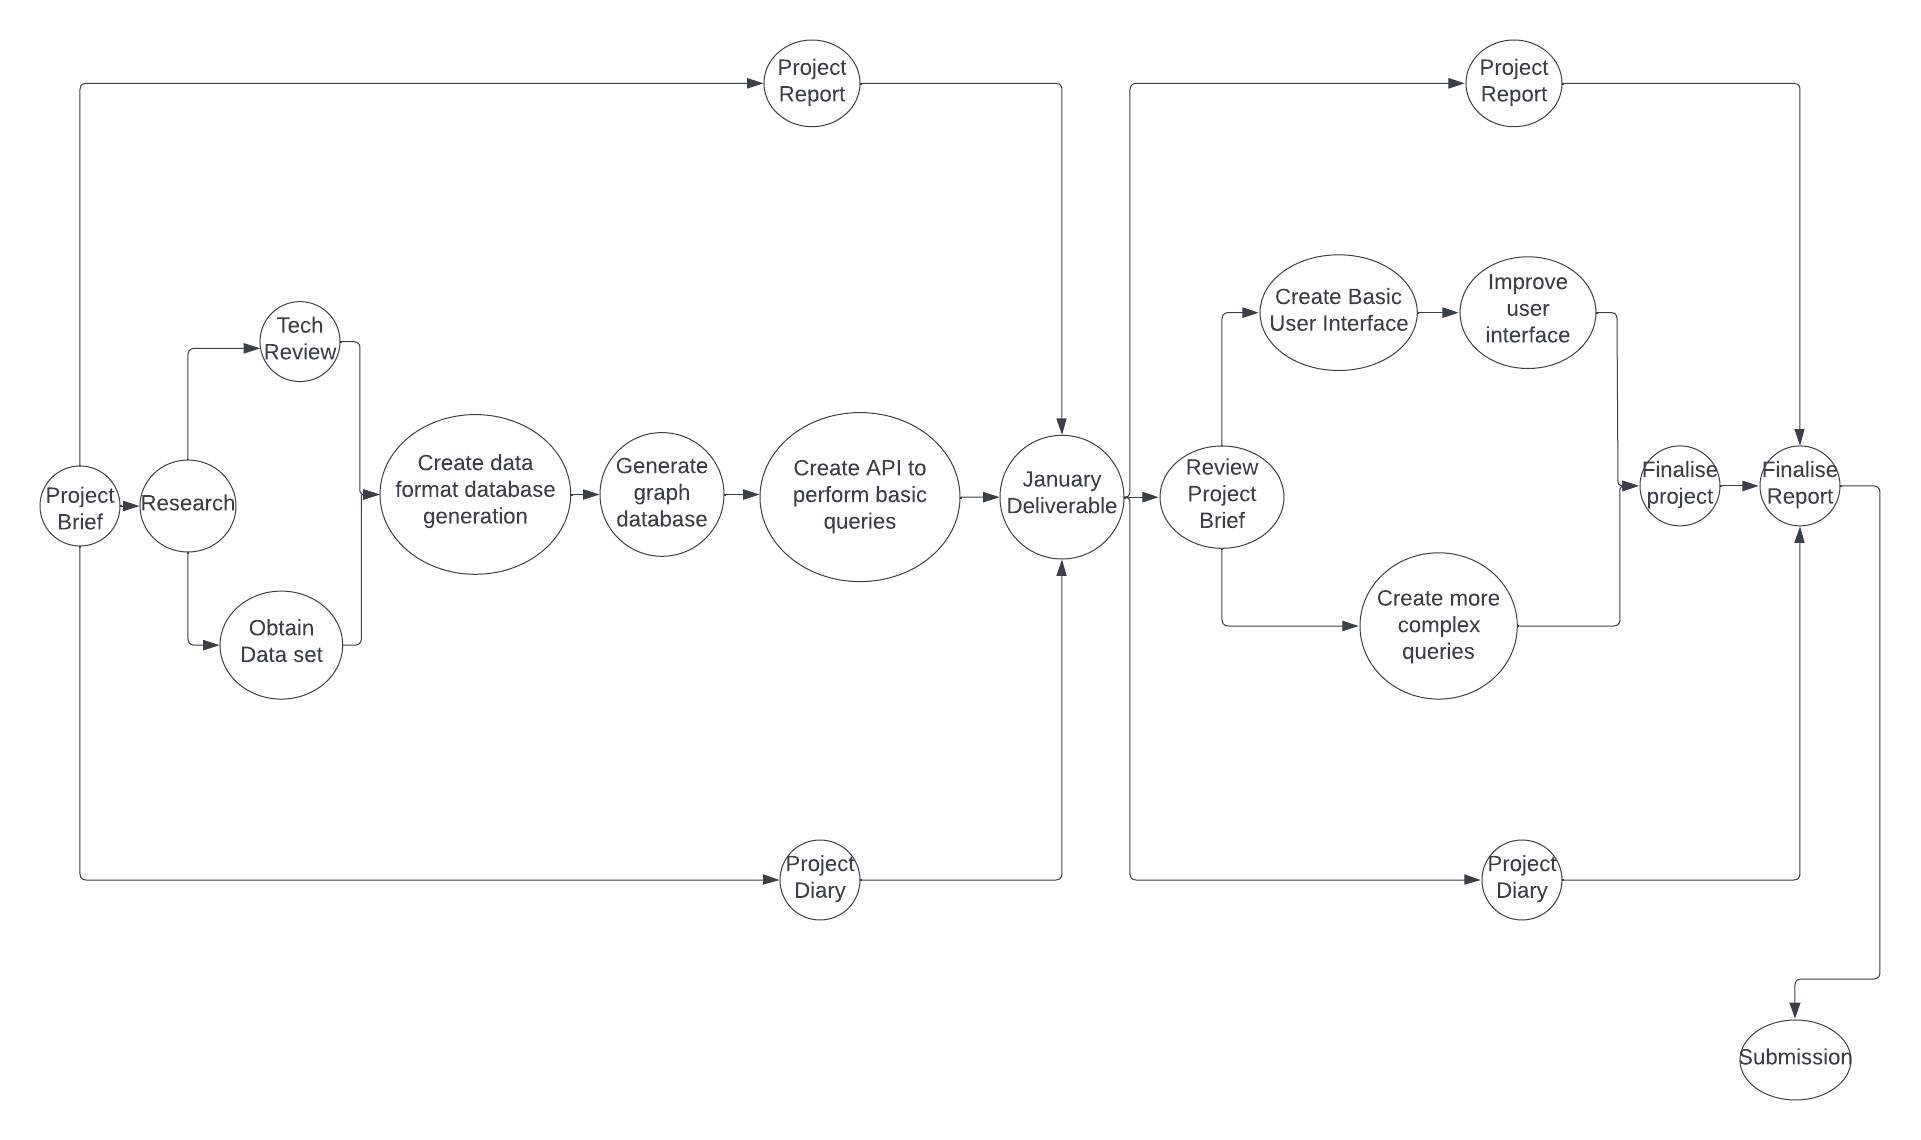
\includegraphics[angle=90,scale=0.7]{PERT}
\end{figure}